%
% File: chap02.tex
%
\let\textcircled=\pgftextcircled
\chapter{Results}
\label{chap:result}

\initial{T}his chapter presents the results obtained during the experiment performed on September 21st, 2016. It presents the subcritical multiplication factor measurements and deduces the number of fuel rods needed to reach criticality.

\section{Subcritical multiplication factor}

The subcritical multiplication factor, $M$, is calculated using the NM1000 raw measurements. Since the neutron flux varies during the time of the measurement, a comprehensive chunk of data is recorded and averaged. Some measurements have been done before the reactor was fully stabilized, but it falls within the calculation uncertainties. Tables~\ref{tab:nm100_rawdata} and~\ref{tab:nm1000_avg} presents the raw results from the NM1000, and table~\ref{tab:critpred} calculates the subcritical multiplication factor and the updated criticality prediction.

\begin{table}[!htb]
    \centering
    \begin{tabular}{cccc}
        Core inventory (\# fuel rods) & Average count rate & $\frac{1}{M}$ & Predictive critical core inventory \\ \hline\hline
        112 & 0.76  & 0.20 &     \\
        115 & 1.10  & 0.14 & 122 \\
        118 & 1.85  & 0.08 & 122 \\
        120 & 2.62  & 0.06 & 123 \\
        122 & 3.49  & 0.04 & 124 \\
        123 & 4.87  & 0.03 & 124 \\
        124 & 7.28  & 0.02 & 125 \\
        125 & 12.18 & 0.01 & 125
    \end{tabular}
    \caption{$\frac{1}{M}$ calculation and criticality prediction}\label{tab:critpred}
\end{table}

Fitting this data linearly should give us, at the intersection with the x-axis -- that is, when M is infinite and thus the core is critical -- the amount of fuel rods needed in the core. One can see on figure~\ref{fig:1overM} that the linearity is debatable, with only an $R^2$ of 95\%. As a reminder, appendix~\ref{app:app04} goes into more details for the calculation of $R^2$. This is expected, since not all the fuel rods have the same worth, some being more irradiated than other, due to their position or time spent in the core, or their initial uranium mass for example.

\begin{figure}[t!]
	\centering
	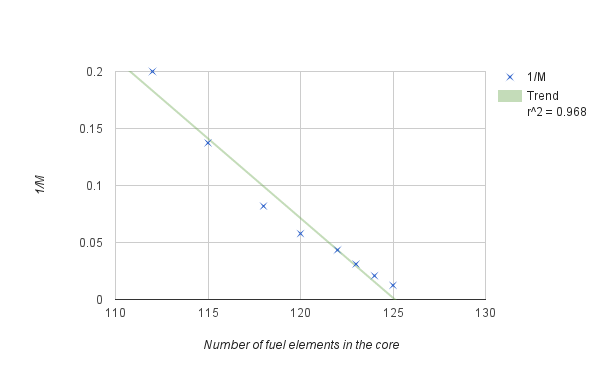
\includegraphics[height=0.4\textheight]{fig02/1overM.png}
	\mycaption[$\frac{1}{M}$ as a function of the number of fuel rods in the core]{$\frac{1}{M}$ as a function of the number of fuel rods in the core.}
	\label{fig:1overM}
\end{figure}

One can see the evolution of the prediction as a function of the number of fuel rods in the core on figure~\ref{fig:prediction}. Keeping in mind that the actual criticality was achieved with 126 fuel rods compared to a full core of 127 rods, one can see that the estimates were lower. \emph{That is good}. Indeed, this means that the approach to criticality was made, by design, in a very conservative way. The method told the operators that less fissile material was needed to achieve criticality, which allowed for a slower reload and no unexpected criticality incident.


\begin{figure}[t!]
	\centering
	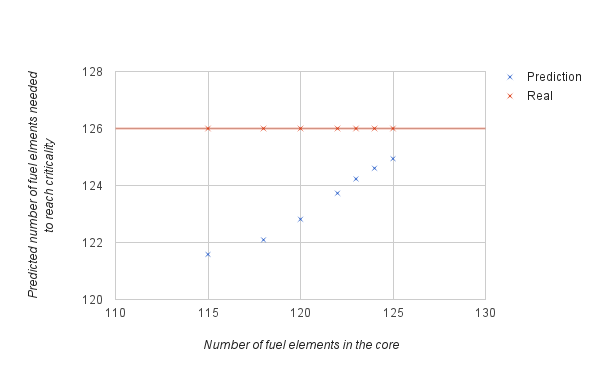
\includegraphics[height=0.4\textheight]{fig02/prediction.png}
	\mycaption[Evolution of the criticality prediction]{Evolution of the criticality prediction.}
	\label{fig:prediction}
\end{figure}
